% Options for packages loaded elsewhere
\PassOptionsToPackage{unicode}{hyperref}
\PassOptionsToPackage{hyphens}{url}
\PassOptionsToPackage{dvipsnames,svgnames,x11names}{xcolor}
%
\documentclass[
  number,
  preprint,
  3p]{elsarticle}

\usepackage{amsmath,amssymb}
\usepackage{lmodern}
\usepackage{iftex}
\ifPDFTeX
  \usepackage[T1]{fontenc}
  \usepackage[utf8]{inputenc}
  \usepackage{textcomp} % provide euro and other symbols
\else % if luatex or xetex
  \usepackage{unicode-math}
  \defaultfontfeatures{Scale=MatchLowercase}
  \defaultfontfeatures[\rmfamily]{Ligatures=TeX,Scale=1}
\fi
% Use upquote if available, for straight quotes in verbatim environments
\IfFileExists{upquote.sty}{\usepackage{upquote}}{}
\IfFileExists{microtype.sty}{% use microtype if available
  \usepackage[]{microtype}
  \UseMicrotypeSet[protrusion]{basicmath} % disable protrusion for tt fonts
}{}
\makeatletter
\@ifundefined{KOMAClassName}{% if non-KOMA class
  \IfFileExists{parskip.sty}{%
    \usepackage{parskip}
  }{% else
    \setlength{\parindent}{0pt}
    \setlength{\parskip}{6pt plus 2pt minus 1pt}}
}{% if KOMA class
  \KOMAoptions{parskip=half}}
\makeatother
\usepackage{xcolor}
\setlength{\emergencystretch}{3em} % prevent overfull lines
\setcounter{secnumdepth}{5}
% Make \paragraph and \subparagraph free-standing
\ifx\paragraph\undefined\else
  \let\oldparagraph\paragraph
  \renewcommand{\paragraph}[1]{\oldparagraph{#1}\mbox{}}
\fi
\ifx\subparagraph\undefined\else
  \let\oldsubparagraph\subparagraph
  \renewcommand{\subparagraph}[1]{\oldsubparagraph{#1}\mbox{}}
\fi


\providecommand{\tightlist}{%
  \setlength{\itemsep}{0pt}\setlength{\parskip}{0pt}}\usepackage{longtable,booktabs,array}
\usepackage{calc} % for calculating minipage widths
% Correct order of tables after \paragraph or \subparagraph
\usepackage{etoolbox}
\makeatletter
\patchcmd\longtable{\par}{\if@noskipsec\mbox{}\fi\par}{}{}
\makeatother
% Allow footnotes in longtable head/foot
\IfFileExists{footnotehyper.sty}{\usepackage{footnotehyper}}{\usepackage{footnote}}
\makesavenoteenv{longtable}
\usepackage{graphicx}
\makeatletter
\def\maxwidth{\ifdim\Gin@nat@width>\linewidth\linewidth\else\Gin@nat@width\fi}
\def\maxheight{\ifdim\Gin@nat@height>\textheight\textheight\else\Gin@nat@height\fi}
\makeatother
% Scale images if necessary, so that they will not overflow the page
% margins by default, and it is still possible to overwrite the defaults
% using explicit options in \includegraphics[width, height, ...]{}
\setkeys{Gin}{width=\maxwidth,height=\maxheight,keepaspectratio}
% Set default figure placement to htbp
\makeatletter
\def\fps@figure{htbp}
\makeatother

\usepackage{booktabs}
\usepackage{caption}
\usepackage{longtable}
\makeatletter
\makeatother
\makeatletter
\makeatother
\makeatletter
\@ifpackageloaded{caption}{}{\usepackage{caption}}
\AtBeginDocument{%
\ifdefined\contentsname
  \renewcommand*\contentsname{Table of contents}
\else
  \newcommand\contentsname{Table of contents}
\fi
\ifdefined\listfigurename
  \renewcommand*\listfigurename{List of Figures}
\else
  \newcommand\listfigurename{List of Figures}
\fi
\ifdefined\listtablename
  \renewcommand*\listtablename{List of Tables}
\else
  \newcommand\listtablename{List of Tables}
\fi
\ifdefined\figurename
  \renewcommand*\figurename{Figure}
\else
  \newcommand\figurename{Figure}
\fi
\ifdefined\tablename
  \renewcommand*\tablename{Table}
\else
  \newcommand\tablename{Table}
\fi
}
\@ifpackageloaded{float}{}{\usepackage{float}}
\floatstyle{ruled}
\@ifundefined{c@chapter}{\newfloat{codelisting}{h}{lop}}{\newfloat{codelisting}{h}{lop}[chapter]}
\floatname{codelisting}{Listing}
\newcommand*\listoflistings{\listof{codelisting}{List of Listings}}
\makeatother
\makeatletter
\@ifpackageloaded{caption}{}{\usepackage{caption}}
\@ifpackageloaded{subcaption}{}{\usepackage{subcaption}}
\makeatother
\makeatletter
\@ifpackageloaded{tcolorbox}{}{\usepackage[many]{tcolorbox}}
\makeatother
\makeatletter
\@ifundefined{shadecolor}{\definecolor{shadecolor}{rgb}{.97, .97, .97}}
\makeatother
\makeatletter
\makeatother
\journal{Quaternary International}
\ifLuaTeX
  \usepackage{selnolig}  % disable illegal ligatures
\fi
\usepackage[]{natbib}
\bibliographystyle{elsarticle-num}
\IfFileExists{bookmark.sty}{\usepackage{bookmark}}{\usepackage{hyperref}}
\IfFileExists{xurl.sty}{\usepackage{xurl}}{} % add URL line breaks if available
\urlstyle{same} % disable monospaced font for URLs
\hypersetup{
  pdftitle={The Fremont Frontier},
  pdfauthor={Kenneth B. Vernon; Peter M. Yaworsky; Weston McCool; Jerry D. Spangler; Simon Brewer; Brian F. Codding},
  pdfkeywords={Ideal Free Distribution, Great Basin, Paleoclimate
Reconstruction},
  colorlinks=true,
  linkcolor={blue},
  filecolor={Maroon},
  citecolor={Blue},
  urlcolor={Blue},
  pdfcreator={LaTeX via pandoc}}

\setlength{\parindent}{6pt}
\begin{document}

\begin{frontmatter}
\title{The Fremont Frontier \\\large{Living at the Margins of Maize
Farming} }
\author[1]{Kenneth B. Vernon%
\corref{cor1}%
}
 \ead{Kenneth.Vernon@colorado.edu} 
\author[2,3]{Peter M. Yaworsky%
%
}

\author[4]{Weston McCool%
%
}

\author[4]{Jerry D. Spangler%
%
}

\author[5,6]{Simon Brewer%
%
}

\author[4,6]{Brian F. Codding%
%
}


\affiliation[1]{organization={},addressline={Center for Collaborative
Synthesis in Archaeology, Institute of Behavioral Science, University of
Colorado, Boulder, 1440 15th Street, Boulder, CO 80302},postcodesep={}}
\affiliation[2]{organization={},addressline={Department of Culture and
Heritage Studies, School of Culture and Society, Aarhus University,
Moesgård Allé 20, building 4216, 8270 Højbjerg, Denmark},postcodesep={}}
\affiliation[3]{organization={},addressline={Center for Biodiversity
Dynamics in a Changing World, Department of Biology, Aarhus University,
Ny Munkegade 114-116, 8000 Aarhus C, Denmark},postcodesep={}}
\affiliation[4]{organization={},addressline={University of Utah
Department of Anthropology, 260 S. Central Campus Drive, RM 4625, Salt
Lake City, UT 84112},postcodesep={}}
\affiliation[5]{organization={},addressline={University of Utah
Department of Geography, 260 S. Central Campus Drive, RM 4625, Salt Lake
City, UT 84112},postcodesep={}}
\affiliation[6]{organization={},addressline={University of Utah Global
Change and Sustainability Center, 115 South 1460 East, RM 234 FASB, Salt
Lake City, UT 84112},postcodesep={}}

\cortext[cor1]{Corresponding author}






        
\begin{abstract}
The Fremont provide an important case study to examine the resilience of
ancient farmers to climatic downturns, for they lived at the far
northern margin of intensive maize agriculture in the American West,
where the constraints on maize production are made abundantly clear.
Using a tree-ring and simulation-based reconstruction of average annual
precipitation and maize growing degree days, along with cost-distance to
perennial streams, we model spatial variability in Fremont site density
in the eastern Great Basin. The results of our analysis have
implications for defining the ecological envelope in which farming is a
viable strategy across this arid region and can be used to predict where
and why maize farming strategies might evolve and eventually collapse as
climate changes over time.
\end{abstract}





\begin{keyword}
    Ideal Free Distribution \sep Great Basin \sep 
    Paleoclimate Reconstruction
\end{keyword}
\end{frontmatter}
    \ifdefined\Shaded\renewenvironment{Shaded}{\begin{tcolorbox}[boxrule=0pt, interior hidden, breakable, sharp corners, enhanced, borderline west={3pt}{0pt}{shadecolor}, frame hidden]}{\end{tcolorbox}}\fi

\hypertarget{introduction}{%
\section{Introduction}\label{introduction}}

Archaeological populations of subsistence maize farmers known
collectively as ``the Fremont'' lived at the far northern periphery of
maize farming in western North America, in an area encompassing much of
the modern state of Utah north of the Virgin and Colorado Rivers, from
roughly 2000 to 700 years BP \citep{madsen1989, madsen1998}. That the
Fremont managed to thrive for as long as they did in this part of the
world poses an interesting question, for conditions there are extremely
harsh and inhospitable for maize farming. Archaeologists interested in
that question have typically focused on strategies directly related to
farming and subsistence, like irrigation methods, trade, and seasonal
high elevation hunting
\citep[e.g.,][]{barlow2008, boomgarden2019, janetski2002, hart2021, madsen1998, metcalfe1985, patterson2010, spangler1993, morgan2012}.
Here, however, we come at the problem from a slightly different angle.
We seek to understand not so much \emph{what} they did to make farming
effective, but \emph{where} they chose to do it, and why they chose
those places over others \citep[e.g.,][]{bocinsky2014, thomson2020}.
Those are not entirely separate questions, of course, as they trade-off
each other, but we think a geographic analysis can actually help
illuminate some of the costs and benefits of the other strategies
adopted by the Fremont. A geographic or spatial model will also help us
to investigate the ways that climate change might have structured those
costs and benefits, and by extension the settlement decisions of Fremont
farmers, which we consider a long-term record of human adaptation to
climate change.

As a test case, we focus on those Fremont living in the eastern Great
Basin of western Utah, which we refer to as the western Fremont (see
Figure~\ref{fig-overview}). The extreme desert conditions that the
western Fremont adapted to provide a useful backdrop for exploring
Fremont settlement, for variation in that environment exhibits abrupt
and quite dramatic changes over short distances of space and time, thus
heightening the differences between areas the western Fremont did and
did not occupy. We explore those differences from a socio-ecological
perspective, focusing on dynamic interactions between competing
individuals on the one hand and individuals and their environment on the
other \citep{bird2006, kennett2006a}. This dynamic is captured nicely by
the Ideal Free Distribution model from Behavioral Ecology, as it
represents individual decisions about where to live as a choice between
habitats whose benefits to the individual may be constrained by what
other individuals are doing. The technical term for these benefits is
`suitability', which the IFD defines as some function of both the
habitat's intrinsic or pristine environmental quality and its current
population size \citep{fretwell1969, codding2015, winterhalder2010}. The
fundamental assumption underlying the IFD is that individuals will
behave optimally, that they will choose to settle the habitat with the
highest suitability first, meaning the one that offers them the greatest
ratio of benefits to costs relative to the available alternatives.

Assuming that western Fremont individuals were adept at responding to
variation in their local ecology, in particular, that they optimized
their choice of habitats, we can use an empirical or inductive species
distribution model of Fremont sites to reconstruct the ecological niche
for maize farming \citep{vernon2021, yaworsky2020, elith2009}. This is
sometimes referred to as ecological niche modeling. The basic idea here
is that we can look at the distribution of Fremont sites as a reliable
indicator of the sorts of available environmental conditions that would
best promote maize farming in an arid landscape. In effect, we are
helping ourselves to a little reverse engineering of the archaeological
record \citep{dennett1995}. We are assuming that whatever strategy -
whatever habitat - the Fremont chose was the best alternative available
to them, not in any absolute sense, of course, just the best given the
constraints and trade-offs Fremont farmers faced in those environments
\citep{jochim2022}. In other words, we are treating their settlement
decisions themselves as maize farming adaptations.

\begin{figure}

{\centering 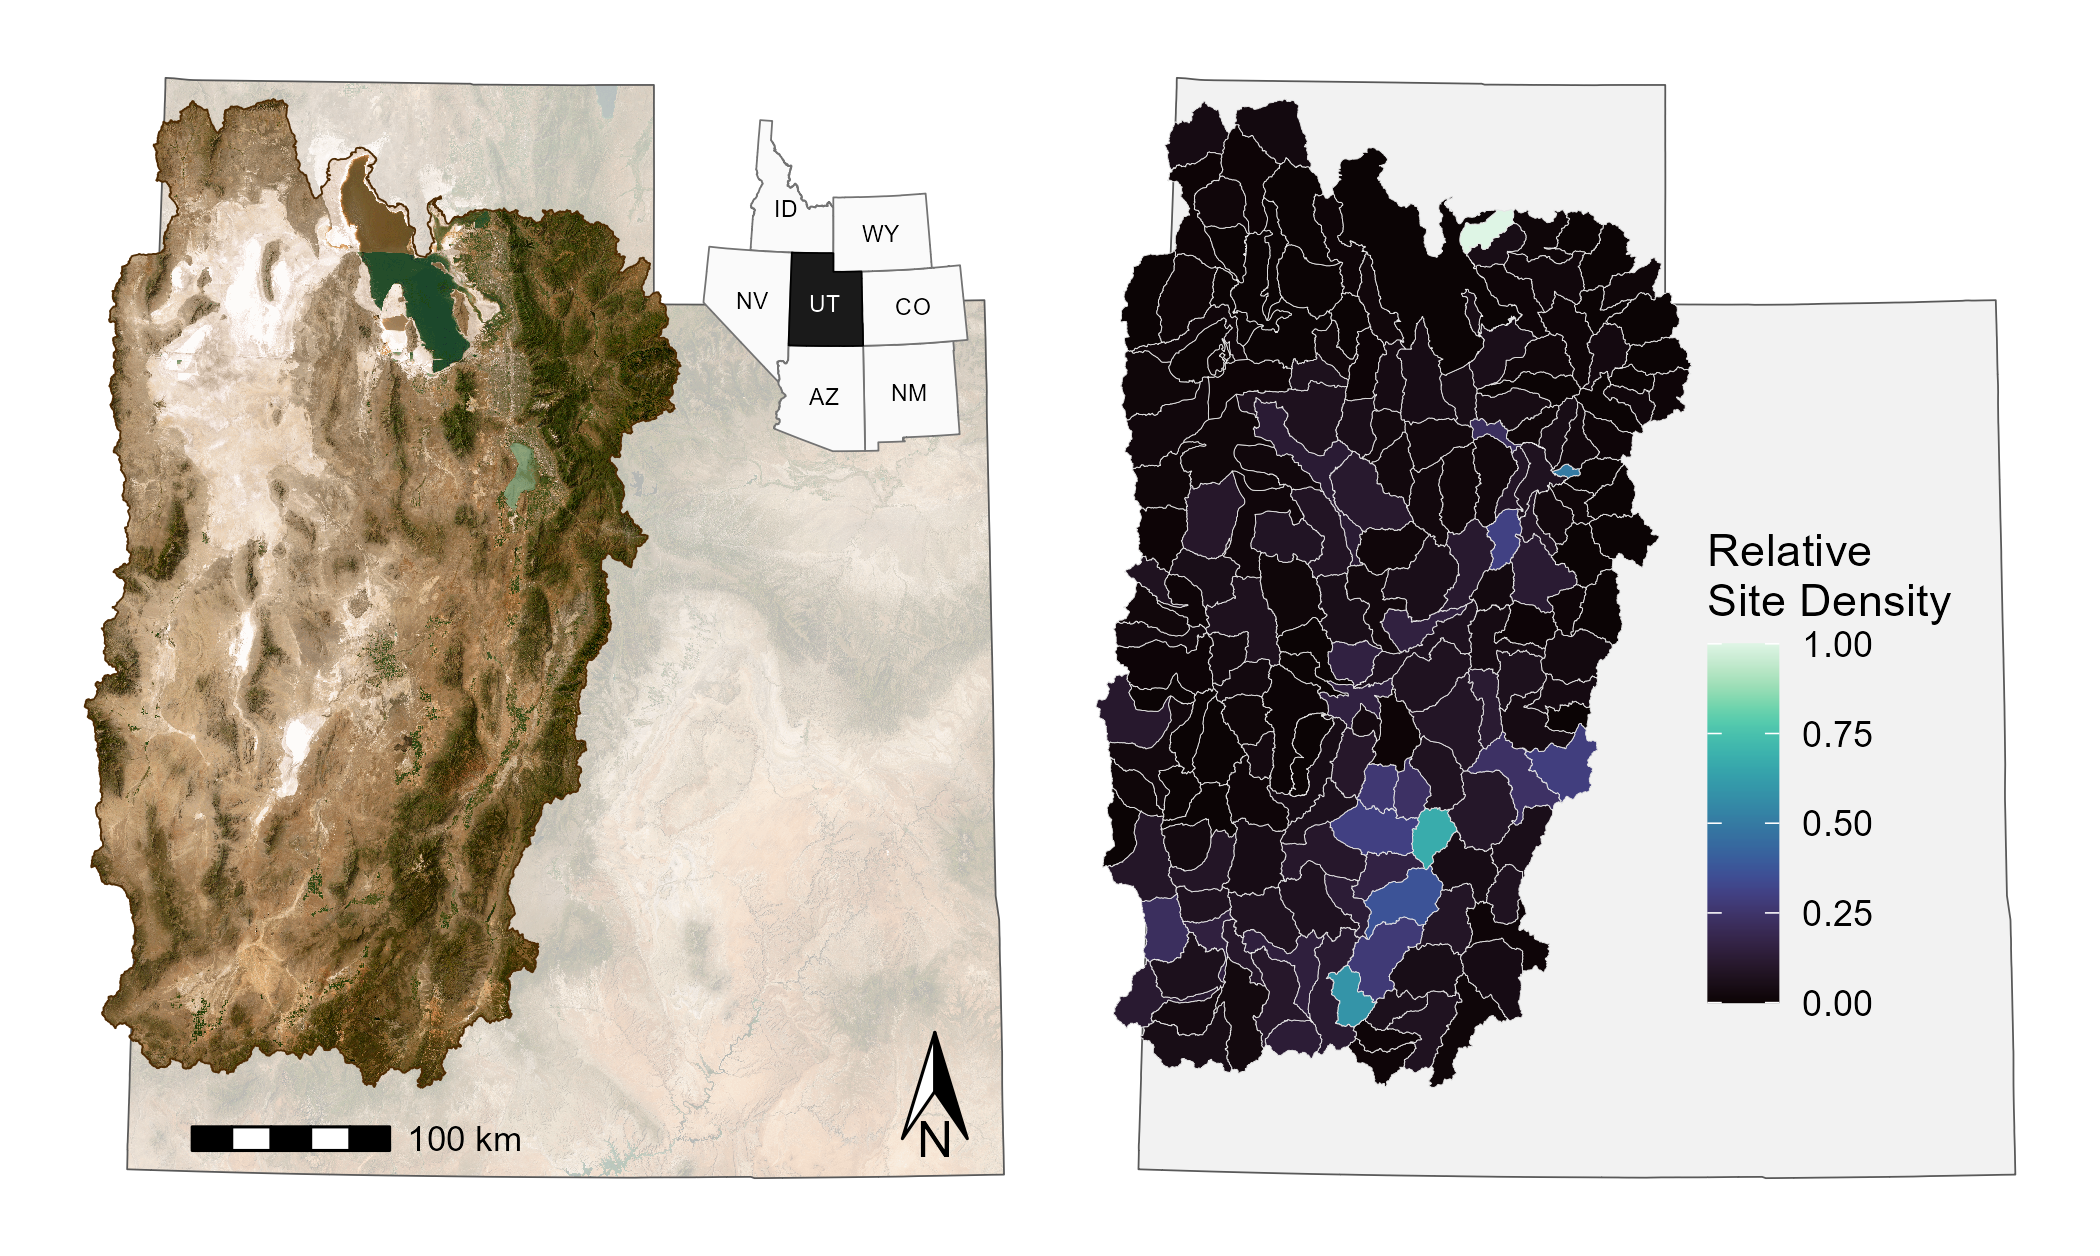
\includegraphics[width=6in,height=\textheight]{../figures/overview.png}

}

\caption{\label{fig-overview}On the left is an overview map showing the
project area with modern satellite imagery. Dark green colors represent
high elevation, high precipitation areas. The large beige area in the
northwest is the Bonneville Basin. What remains of the Great Salt Lake
can be seen just west of Salt Lake City. For visualization purposes, the
map on the right shows the relative density of archaeological sites (see
the section on site data below for details on how we calculate relative
density). Please note that although the map appears to show many empty
watersheds, most do in fact contain archaeological sites, just at
extremely low densities.}

\end{figure}

\hypertarget{background}{%
\section{Background}\label{background}}

\hypertarget{the-fremont}{%
\subsection{The Fremont}\label{the-fremont}}

Archaeologists have nominated a number of artifact types and artifact
properties as candidate traits to distinguish the Fremont from their
neighbors in space and time, including metates with secondary grinding
surfaces, large semi-subterranean pithouses, various clay figurines,
trapezoidal rock art, one-rod-and-bundle basketry, painted white and
corrugated gray ceramics, and elongated corner-notched arrow points
\citep{madsen1998}. None of these, however, nor any combination of them,
has yet proven up to the task of bringing these diverse people under a
single, all-encompassing definition \citep{madsen1998}. Nevertheless,
the Fremont do stand out, especially at their population apex roughly
1000 years BP.

Around this time, the Fremont likely reached their greatest geographic
extent, inhabiting an area that encompassed most of the modern state of
Utah \citep{janetski2011}, with varying levels of support for
occupations in Idaho \citep{dean1992prehistoric}, Nevada
\citep{hockett1998}, Colorado \citep{baker1999}, and Wyoming
\citep{hakiel1987archery, smith1992fremont}. These modern political
boundaries roughly overlap with the eastern Great Basin and Colorado
Plateau physiographic provinces.

\begin{figure}

{\centering 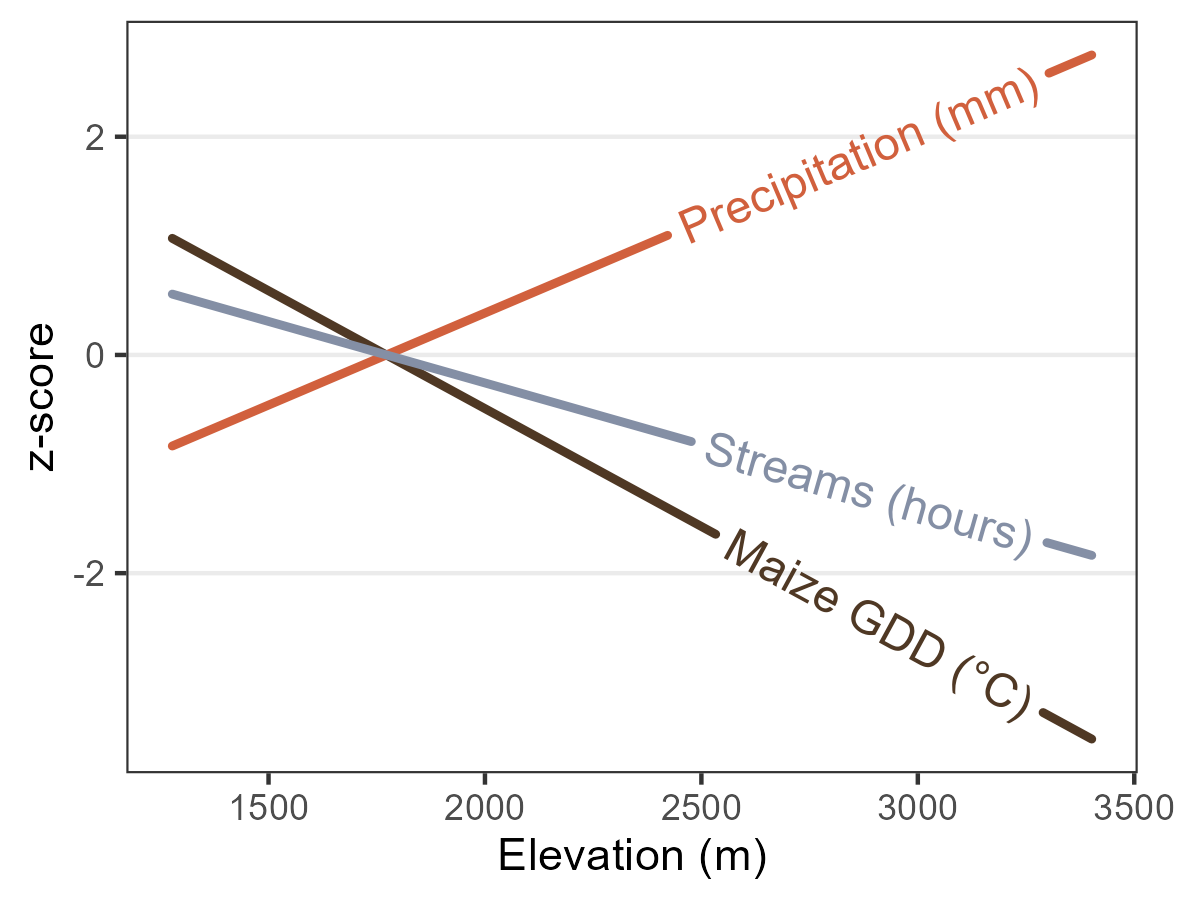
\includegraphics[width=4in,height=\textheight]{../figures/elevation-everything.png}

}

\caption{\label{fig-elevation}Linear responses of average water-year
precipitation (mm), average growing-season maize gdd (C), and
cost-distance to streams (hours) to changes in elevation (m). See
methods for how these values were calculated and results for more
details.}

\end{figure}

A basin and range topography dominates the landscape of the Great Basin,
with large, dry valleys and endorheic basins punctuated by north-south
trending mountain ranges. Changes in elevation in this setting are quite
dramatic, on the order of several thousand meters over a short east-west
transect. As elevation drives virtually every climatological process in
the region, the local ecology is characterized by equally dramatic
extremes \citep{billings1951, grayson2011}. As shown in
Figure~\ref{fig-elevation}, net water-year precipitation in the eastern
Great Basin tends to increase with elevation, while maize growing degree
days (GDD) over the growing-season tends to decrease. An important
trade-off thus exists between temperature and precipitation, with warmer
and drier conditions at lower elevations and cooler and wetter
conditions at higher elevations.

These are the environments into which the Fremont first emerged in
western Utah. Models for describing their origins, while diverse, tend
to fall into the familiar categories of migration and diffusion. Where
models of the former migration variety insist that Ancestral Puebloan
farmers migrated northward from the US Southwest, bringing with them
drought-tolerant maize varieties and maize farming
\citep{madsen1975, kidder1924}, models of the latter diffusion variety
suggest that the Fremont first emerged within these areas as local
Archaic populations transitioned away from mobile foraging, adopting
semi-sedentary agricultural practices from the southwest in a piecemeal
fashion over several hundred years \citep{jennings1978, winter1974}.
While archaeologists have marshaled an impressive array of arguments and
counter-arguments for these two classes of models, a general consensus
appears to be coalescing around the idea that the truth lies somewhere
in between, that the interaction between a nascent Archaic population
existing at extremely low population levels and a burgeoning community
of migrant farmers together produced the complex we now call the Fremont
\citep{patterson2015, simms1986, spangler1993, spangler2000, spangler2013}.

Models that try to explain \emph{why} Fremont maize farmers emerged in
the far northern periphery of the US Southwest tend to agree - more or
less - that at some point farming became a more economical alternative
to foraging in the region. Where they differ, it is in whether things
got better for farming starting roughly 2000 years BP
\citep{benson2011, coltrain2002, matson1988} or worse for foraging
\citep{barlow2002, broughton2010, cannon2000, cannon2001}. In support of
the \emph{farming-more-better} model, archaeologists draw on evidence
for a suite of favorable climatic conditions that came together around
1600 years BP, including warmer temperatures and increased precipitation
(both winter and summer), as well as the expansion of grasslands
\citep{grayson2006, hemphill1995, rhode2000}. The greatest expansion of
the Fremont, in fact, occurred around 1000 years BP, around the time the
Medieval Climate Anomaly (MCA) introduced warmer summer temperatures
that would have increased the intensity of summer monsoons in the
southwest, pushing them further north into the Great Basin and onto the
Colorado Plateau \citep{grayson2006}, a pattern reflected in numerous
tree ring records
\citep[e.g.,][]{graybill1990, leavitt1994, stine1990, salzer2014},
though some complications do exist for this suggested pattern
\citep{hart2021}.

In response to these sorts of arguments, those who favor the
\emph{foraging-more-worse} model \citep{hart2021, barlow2002} argue that
conditions promoting maize farming would also tend to make foraging a
more productive strategy. Plus, farming is an extremely costly endeavor,
especially when compared to foraging, including lots of upfront
investment of time and energy, so improving conditions favorable to
maize agriculture are not by themselves sufficient to explain its
origins. To fill that lacuna, archaeologists point to accumulating
evidence suggesting that the Fremont transition to agriculture
accompanied periods of sustained population growth
\citep{barlow2008, codding2021, spangler2013} that likely resulted in
the depressed availability of wild resources
\citep{barlow2002, janetski1997, simms1986}. So, demographic pressure
reduced the efficiency of foraging strategies, thus making maize
agriculture the optimal strategy. And that, in turn, led the Fremont to
adopt farming as their primary mode of subsistence.

Once they entered the farming niche, the Fremont quickly developed
several adaptations for coping with the marginal and stochastic
conditions in the eastern Great Basin and the Colorado Plateau, the most
important almost certainly being irrigation (for more on this, see the
discussion). On the Colorado Plateau, the eastern Fremont settled deep
within the steep canyons and washes that flanked the tributaries of
major rivers like the Green and Yampa {[}\citep{yaworsky2021}; see also,
Yaworsky this issue{]}, in places like Nine Mile Canyon
\citep{spangler1993} and Range Creek Canyon \citep{hart2021}. In the
eastern Great Basin, the western Fremont chose to settle on open,
alluvial fans and stream terraces along the lower slopes of most ranges
\citep{janetski2000, madsen1998, simms2008}, at places like Nephi Mounds
\citep{sharrock1967}, Pharo Village \citep{marwitt1968}, Median Village
\citep{marwitt1970}, Evans Mound \citep{berry1972, dodd1982}, and Snake
Rock Village \citep{aikens1967}.

Given the extreme aridity of the west, they were still susceptible to
drought, of course, even in those more suitable areas, with a single
short growing season making agricultural returns highly variable. To
cope with these uncertainties, Fremont farmers may have adopted
additional risk-mitigation strategies like spreading farm plots among
different micro-environments, a technique otherwise known as plot
diversification \citep{spangler1993, spangler2013, patterson2015}. The
Fremont also relied heavily on crop storage both to provide a surplus
during the winter season and to make-up for poor yields
\citep{spangler2019}.

\hypertarget{the-ideal-free-distribution}{%
\subsection{The Ideal Free
Distribution}\label{the-ideal-free-distribution}}

In population ecology, settlement decisions are represented as a choice
between habitats, where each habitat \(i\) has some net biological value
or benefit, known as its suitability (\(S_i\)). Typically, though not
always, this value exhibits negative density dependence, declining as a
function of population size (\(N_i\)), perhaps owing to increased
competition or resource depression. When \(N_i\) is very small, the
suitability of a habitat approaches its pristine or intrinsic quality
(\(Q_i\)), or its gross value independent of all settlement costs
\citep{greene2001}. Together, these parameters suggest a very simple
model of habitat suitability:

\[
S_i = Q_i - f(N_i)
\]

This is known as the Ideal Free Distribution (IFD) model
\citep{fretwell1969}. The IFD model assumes that individuals will choose
habitats that maximize \(S_i\), settling the most suitable habitat first
then shifting to the next most suitable habitat when those become equal,
and thereafter infilling each at an equal rate. The aggregate effect is
a population distributed at equilibrium, meaning suitability is equal
for all habitats. When conditions are ideal (individuals have perfect
knowledge) and free (individuals face no additional costs to
settlement), this distribution will also satisfy the ``input matching''
rule, with populations occurring at larger numbers in habitats with
greater intrinsic value \citep{parker1978}.

Two circumstances provide important exceptions to this simple model. The
first concerns economies of scale, or situations in which \(S_i\)
exhibits positive density dependence. In ecology, these are known as
Allee effects, and they are assumed to occur at low density
\citep{allee1949, fretwell1969}. The second concerns additional
settlement costs, or costs associated with moving from one habitat to
another. This is a violation of the free element of the IFD. When it
occurs, the result is an ideal despotic distribution (IDD)
\citep{fretwell1969}. This has the consequence of reducing the total
population in the more suitable habitat at equilibrium.

Many social and ecological variables may be relevant to defining a
general measure of \(S_i\), but here we are focusing on ecological
determinants of intrinsic habitat quality, \(Q_i\), that are specific to
maize farmers. Our reasoning here is fairly straightforward. If we
assume that the distribution of Fremont populations across habitats is
at equilibrium, then we can combine this concept of maize-specific
suitability with the input matching rule to reconstruct the ranking of
habitats on the basis of ecologically-relevant parameters. That is, it
follows from their being at equilibrium that any observed differences in
population size must be the result of differences in \(Q_i\), that
\(Q_i \approx f(N_i)\) at equilibrium. So, if we have some proxy for
\(N_i\), like the distribution of Fremont sites across habitats, we can
model that value as a function of ecological covariates \(X_i\), then
use the resulting model to reconstruct \(Q_i \approx f(X_i)\), giving us
the maize niche for Fremont farmers, both in geographic and ecological
space.

\hypertarget{materials-and-methods}{%
\section{Materials and Methods}\label{materials-and-methods}}

\hypertarget{the-project-area}{%
\subsection{The Project Area}\label{the-project-area}}

Because we are focusing on the western Fremont, we constrain the current
project area to the eastern Great Basin in western Utah, as shown in
Figure~\ref{fig-overview}, where the Great Basin is defined in the
hydrologic sense using watershed boundaries \citep{grayson2011}. On the
far eastern edge of this region, a series of north-south ranges,
including the Wasatch, Pahvant, and Tushar Mountains, together stand as
the primary physiographic boundaries separating the Great Basin from the
Colorado Plateau. On its far western edge, a series of north-south
ranges straddle the Nevada state line or lie just inside it, including
the Snake Range where Great Basin National Park is located. Its northern
periphery is the Great Salt Lake and the West Desert, its southern
boundary the Pine Valley Mountains that separate the Great Basin from
the Virgin River watershed, just north of St.~George, UT. This is a
region approximately 107,000 km\(^2\) in area, encompassing virtually
all of the Bonneville Basin in western Utah.

These boundaries also serve as geographic borders between the western
Fremont and other contemporaneous populations. Around the Great Salt
Lake and the Utah-Nevada border, Fremont farming gives way to Archaic
populations engaged in intensive foraging modes of subsistence. The
Wasatch Range and Tushar Mountains separate the western from the eastern
Fremont on the Colorado Plateau, and the Pine Valley Mountains serve as
a border between the Fremont and the Virgin Ancestral Puebloan to the
south \citep{simms2008}.

\hypertarget{the-unit-of-analysis}{%
\subsection{The Unit of Analysis}\label{the-unit-of-analysis}}

The unit of analysis for this research is the HUC10 watershed (n = 183),
as defined by the Watershed Boundary Dataset (WBD) developed by the US
Geological Survey and the Natural Resources Conservation Service within
the US Department of Agriculture \citep{usgs2013}. These provide a
spatially-explicit proxy for specifically human habitats in the proposed
study area. There are two reasons for this. First, the topography of the
region is such that the cost of travel between watersheds is often quite
significant. As a consequence, individuals are expected to spend more
time traveling within watersheds than between them, all else being
equal. Second, watersheds are by definition water sinks, funneling all
available run-off into their respective stream networks. Given the
extreme aridity of the proposed project area, this also makes them
critical resource sinks, especially for maize farmers, as watersheds
determine how much water might accumulate at a location, as well as its
potential for irrigation.

Aggregating to the level of the watershed also reduces the computational
burdens of this modeling exercise. In particular, it makes paleoclimate
reconstructions more tractable, as we are only estimating the means
within each watershed through time (see below for details).

\hypertarget{site-data}{%
\subsection{Site Data}\label{site-data}}

To identify Fremont sites in the project area, we rely on site records
and cultural resource reports hosted by the cultural resource
information systems in Nevada (NVCRIS) and Utah (Sego) with permission
from the respective State Historic Preservation Offices. The Sego system
also includes an attribute table with affiliation data that we use to
filter Fremont sites where possible. For a previous project, we also
performed a stratified random sample of all archaeological sites by
county in western Utah and recorded affiliation and other attribute data
from their site forms. For this analysis, we compare the results of that
previous effort with the sites identified by filtering the Sego system
as a form of quality control. The resulting dataset contains 2,248
individual Fremont sites.

These site data include everything from small ceramic scatters to
massive Fremont villages like Five Finger Ridge
\citep{janetski1998, janetski2000}. For this analysis, we assume that
these reflect different levels of population size and settlement
intensity. All else being equal, scatters should follow from shorter
stays by fewer people, villages from longer stays by more people. This
is important because population size correlates with a habitat's total
suitability according to the IFD model, and our attempts to reconstruct
the ecological and geographic borders of the Fremont rely heavily on the
input-matching rule, or the idea that habitats with greater intrinsic
quality will have larger populations at equilibrium. We, therefore,
weight the count of sites in each watershed by the total number of
residential features that they contain (+1 for sites with no features).
So, a site with no residential features counts as one site, a site
consisting of, say, four pithouses counts as four unique sites, and a
site containing a roomblock with seven rooms counts as seven sites. This
brings the total weighted site count to 2,447, with minimum and maximum
values of 0 and 119, respectively.

Figure~\ref{fig-overview} shows the relative density of Fremont sites
across watersheds. The \emph{relative} density refers to the density of
feature-weighted sites (\(D_i = N_i/area_i\)) divided by the maximum
density (\(max\;D\)) across all watersheds, thus scaling the density
estimates to the unit interval {[}0,1{]}. Using the relative density is
just a way of avoiding any implication that we have an independent
estimate of the absolute number of Fremont sites in the area, and not
just an estimate based on a thinned sample.

\hypertarget{environmental-covariates}{%
\subsection{Environmental Covariates}\label{environmental-covariates}}

For this analysis, we use both topographic and climatological
covariates. The topographic covariate is cost-distance to perennial
streams (measured in hours). This provides a coarse grained estimate of
water availability, as well as the potential costs of irrigation. To
calculate this, we first use the R package FedData \citep{bocinsky2020}
to download perennial stream features from the US National Hydrography
Dataset \citep{usgs2022} and a digital elevation model (DEM) from the US
National Elevation Dataset \citep{usgs2022a}. We then apply Campbell's
hiking function \citep{campbell2019} to slope estimates derived from the
DEM using the R package hiker \citep{vernon2021a}. This allows us to
generate estimates of travel time between grid cells in the DEM and then
calculate the accumulated cost of travel from each perennial stream to
any grid cell within each watershed. We then aggregate these values to
the watershed level by taking their mean.

Climate covariates include net water-year precipitation (precipitation,
in millimeters, mm) from October to September and maize growing degree
days (GDD, in Celsius, C) over the growing season from May to September,
as these have a large effect on maize productivity, thus providing
important constraints on the patterns of settlement for those who relied
on maize for subsistence. We caution that GDD is calculated in such a
way as to be insensitive to extreme high and low temperatures (extreme
heat and frost, in effect). It is also conceptually understood to be a
measure of accumulated temperature between the last and first frost-free
days, but in our analysis is calculated using hard start and end dates
of May 1 and September 30, under the assumption that these dates will
roughly coincide with those frost-free days.

\begin{figure}

{\centering 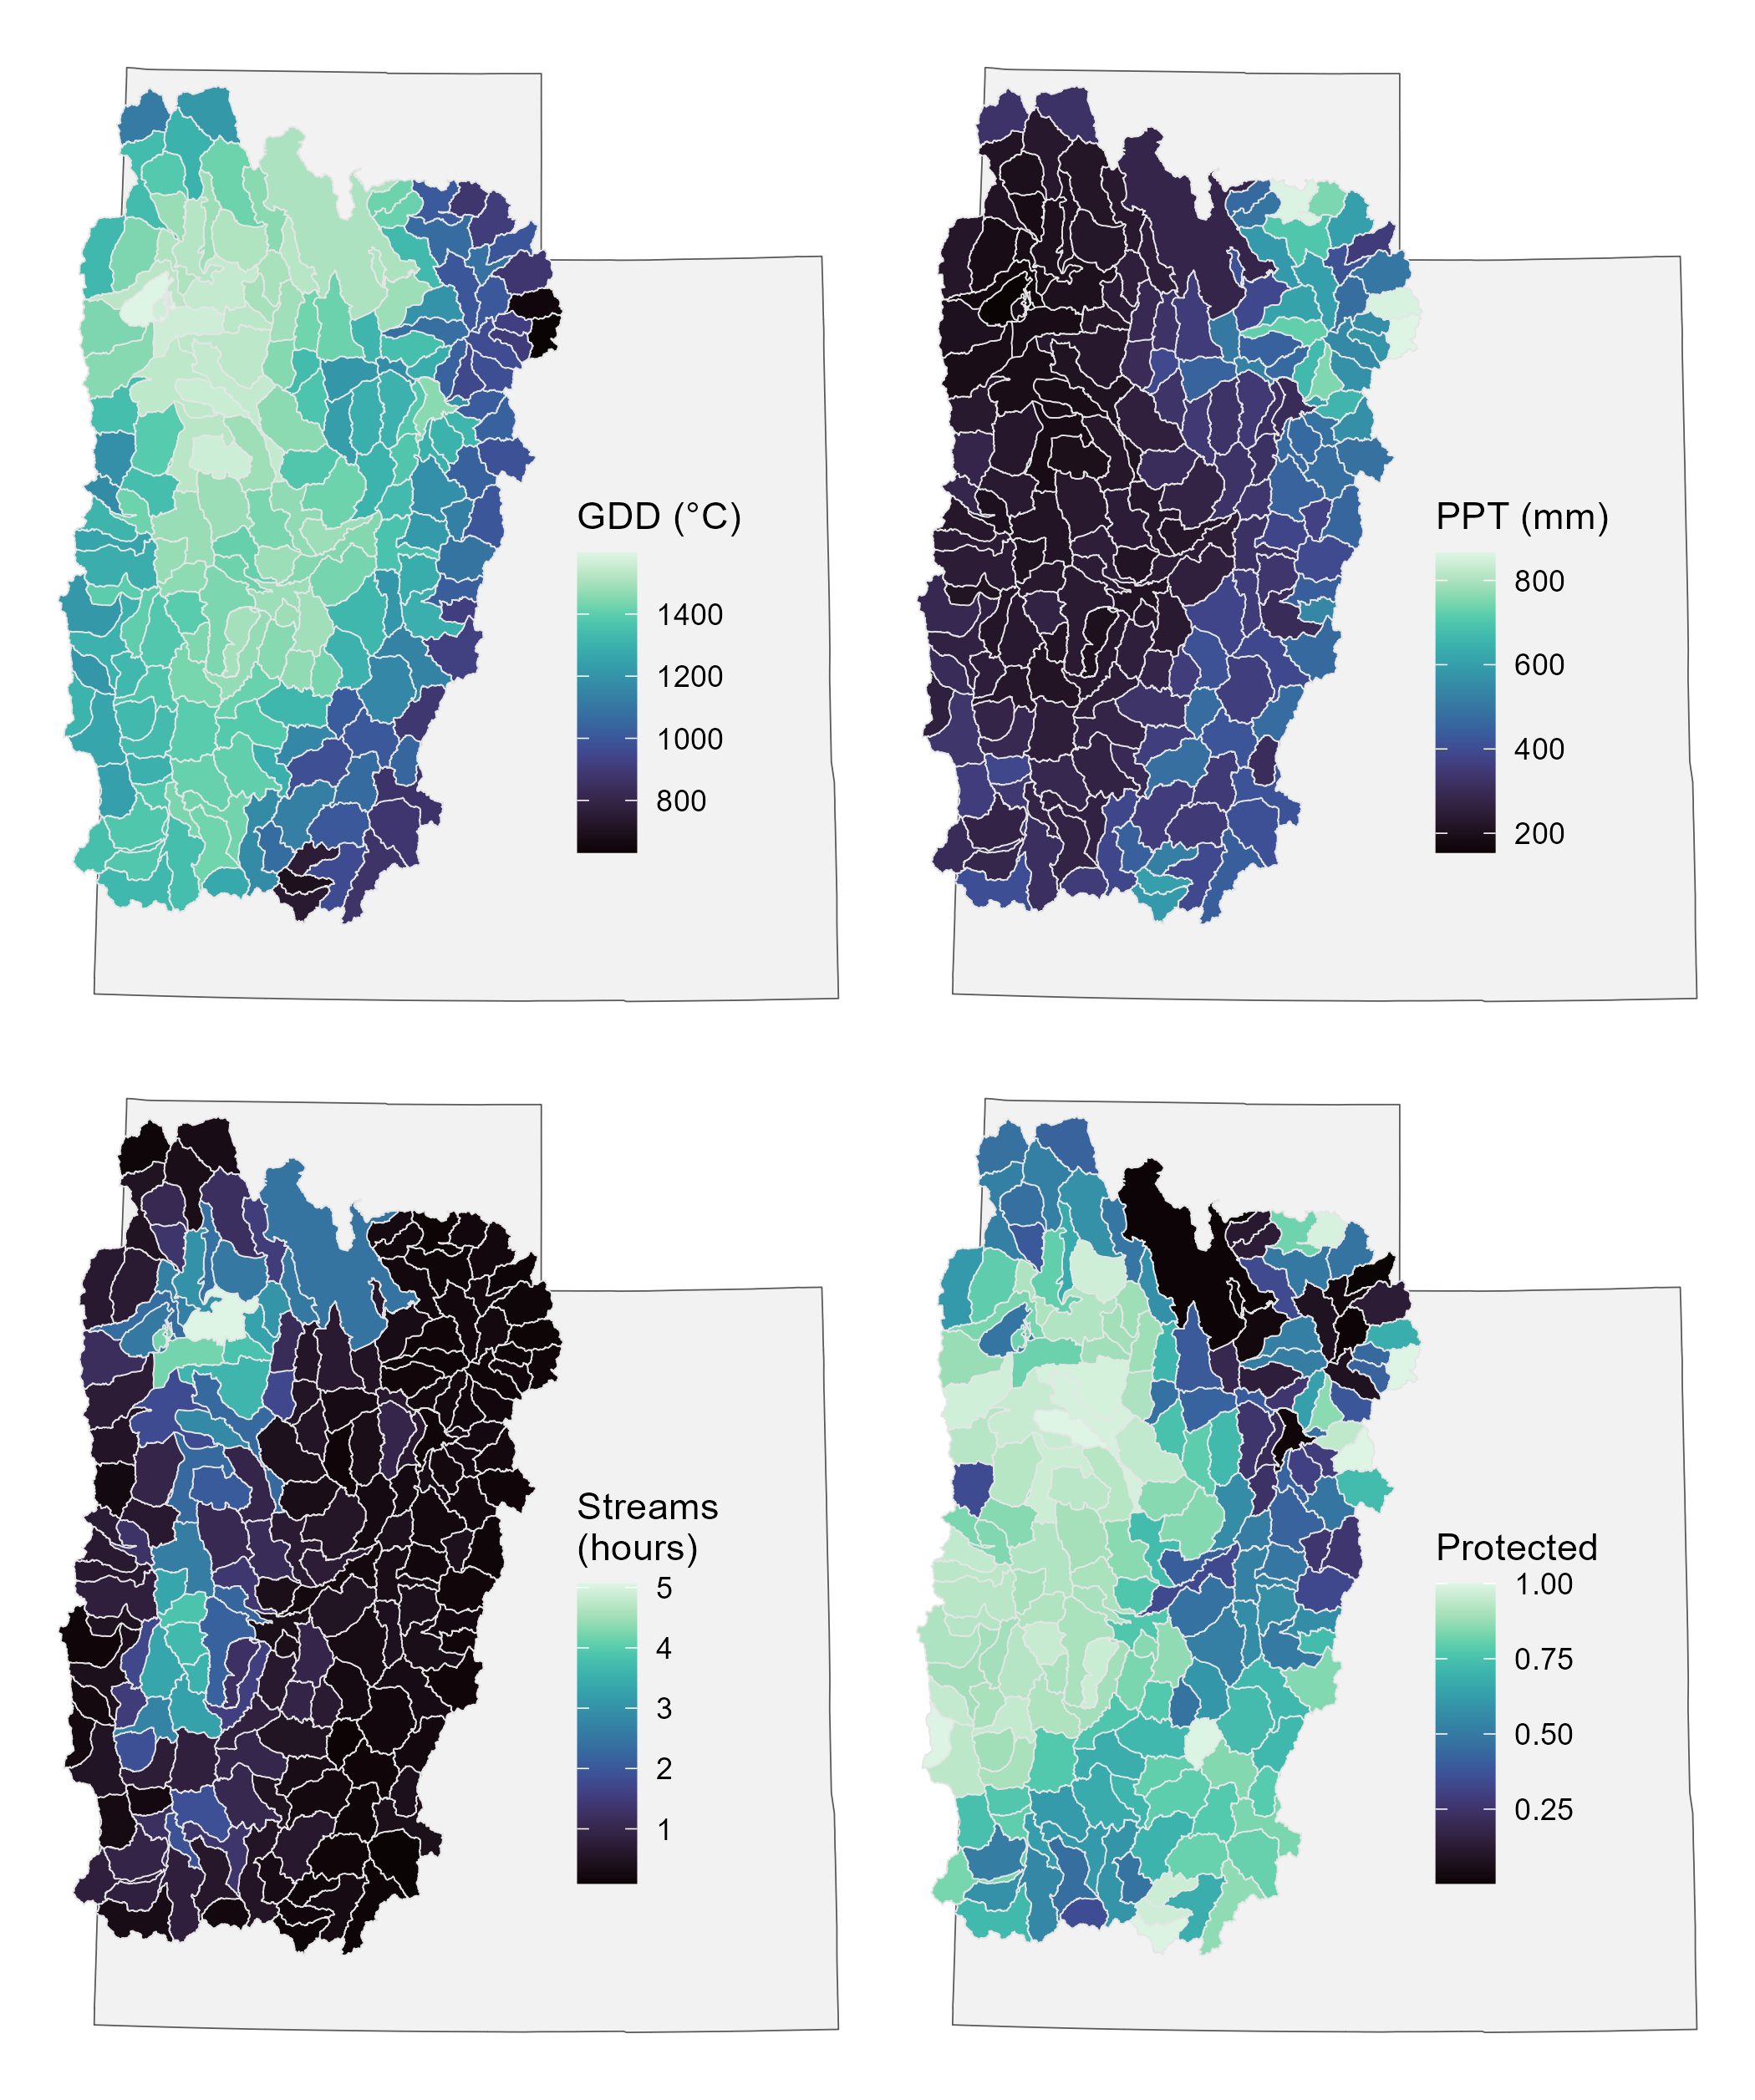
\includegraphics[width=6in,height=\textheight]{../figures/covariates.png}

}

\caption{\label{fig-covariates}Distribution of covariates across
watersheds. These include maize growing degree days (GDD), annual
precipitation (precipitation), and cost-distance to streams (Streams).}

\end{figure}

We hindcast these climate covariates for each watershed and year over
the Fremont sequence from 1550 to 550 years BP (400 to 1400 CE) using
the Correlation Adjusted corRelation (CAR) method implemented in the R
package paleocar \citep{bocinsky2019}. This method, in effect, regresses
modern climate data against the width of younger tree rings, then uses
older rings to predict past climate trends \citep[for further details,
see][]{bocinsky2014, bocinsky2016}. In this case, we use interpolated
precipitation and temperature estimates from the \textasciitilde800 m
resolution PRISM dataset \citep{prismclimategroup2014} and all tree-ring
samples in North America, which were obtained from the International
Tree Ring Database using FedData. For each watershed, we took the median
values of precipitation and GDD over the Fremont sequence.

Figure~\ref{fig-covariates} shows the geographic distributions of these
covariates over watersheds. As these are all in one way or another
driven by elevation, it is reasonable to expect that they will
correlate. As part of the exploratory phase of this analysis, we,
therefore, perform a series of pair-wise tests of correlation measured
using Pearson's R. We also regress the scaled and centered values (or
z-scores) of maize GDD, precipitation, and cost-distance to streams on
elevation using ordinary least squares (OLS). No doubt, this violates
many assumptions of OLS, particularly the identity and independence of
the errors, but explanation was not our main goal with these simple
linear models. We are only trying to get a rough sense of their general
response to changes in elevation, which OLS offers (see
Figure~\ref{fig-elevation}).

Given that our primary covariates all correlate with elevation (reported
below), readers may wonder why we do not simply use elevation in our
main analysis. The reason for this is two-fold. First, using elevation
alone would obscure the trade-off between water availability and
temperature. Second, elevation is not explanatory of settlement
behavior. A maize farmer does not choose a location for farming
\emph{because} it is at, say, 1200 m above sea level. They choose that
location \emph{because} it has the right combination of water
availability and temperature, that is to say, because conditions there
are optimal for maize farming. Were those conditions found at some other
elevation, the farmer would be expected to farm there.

\hypertarget{statistical-modeling-and-model-evaluation}{%
\subsection{Statistical Modeling and Model
Evaluation}\label{statistical-modeling-and-model-evaluation}}

The response variable is a count \(N\) of sites per watershed \(i\), so
it should arise as the result of a Poisson process. Given the trade-offs
outlined above, we also expect it to exhibit a non-linear response to
precipitation, GDD, and cost-distance to streams, so we fit a
generalized additive model (GAM) with a log-link to the data using the R
package mgcv \citep{wood2004}. Although we expect the outcome to be
Poisson distributed, we use a negative binomial distribution here, as
this includes a parameter, \(r\), that can account for potential
dispersion without giving up the inferential benefits of maximum
likelihood.

\[
\begin{aligned}
N_i \sim& \;NB\,(\lambda, r)\\
E\,(N_i) =& \;\lambda_i\\
log\, (\lambda_i) =& \;log\, (area_i) + s(precipitation_i) + streams_i + gdd_i + protected_i
\end{aligned}
\]

Importantly, we add to the model specification a constant offset for the
log of the area of each watershed, in effect making this a model of
population \emph{density}. This is meant to address the idea that larger
watersheds will have more sites just as a matter of chance. While our
model as currently specified includes the intercept, we caution that
such an estimate is not strictly meaningful for this kind of data, as it
assumes that the absolute site counts can be inferred from the sample,
which requires that the sample be unbiased - an implausible condition to
meet. On that note, we also include a parametric term for the proportion
of each watershed classified as federally protected land. This is meant
to address potential sampling biases owing to taphonomic processes
operating on the archaeological record. Notably, for these data, those
are almost entirely the result of Euro-American colonization of the
area, in particular, the impacts of modern farming techniques and the
development of the Wasatch Front as the urban core of the modern state
of Utah. This is a coarse metric, but our expectation is that the
greater the share of a watershed with federal protections, the smaller
the effect of these anthropogenic impacts, the more sites we should
observe.

Model evaluation includes checks for concurvity or non-linear
correlation in the smooth terms of the GAM, as well as a Variance
Inflation Factor test on the parametric or linear terms. We also test
for spatial autocorrelation in the untransformed residuals using Monte
Carlo simulations of Moran's I and incorporate an exponential covariance
matrix to remove that residual autocorrelation. Several smooth terms had
effective degrees of freedom (EDF) equal to one, suggesting no
non-linear response in the data. We, therefore, remove the smooth terms
for those covariates in the final model, as expressed in the formula
above.

All analyses are conducted in the R programming language and environment
\citep{rcoreteam2022}. For details of this analysis, please see the
Supplement.

\hypertarget{results}{%
\section{Results}\label{results}}

\begin{table}

\caption{\label{tbl-results}Model
Results}\begin{minipage}[t]{\linewidth}
\subcaption{\label{tbl-results-1}Parametric Terms }

{\centering 

\setlength{\LTpost}{0mm}
\begin{longtable}{lcccc}
\tabularnewline

\toprule
 & \textbf{exp(Beta)} & \textbf{SE}\textsuperscript{\textit{1}} & \textbf{t} & \textbf{p-value} \\ 
\midrule
Intercept & 0.00 & 1.40 & -7.13 & <0.001 \\ 
Maize GDD & 1.00 & 0.001 & 4.15 & <0.001 \\ 
CD to Streams & 0.67 & 0.156 & -2.57 & 0.011 \\ 
Protected & 4.82 & 0.497 & 3.16 & 0.002 \\ 
\bottomrule
\end{longtable}
\begin{minipage}{\linewidth}
\textsuperscript{\textit{1}}SE = Standard Error\\
\end{minipage}

}

\end{minipage}%
\newline
\begin{minipage}[t]{\linewidth}
\subcaption{\label{tbl-results-2}Smooth Terms }

{\centering 

\begin{longtable}{lcccc}
\tabularnewline

\toprule
 & \textbf{edf} & \textbf{ref.df} & \textbf{F} & \textbf{p-value} \\ 
\midrule
s(Precipitation) & 3.25 & 3.25 & 11.1 & <0.001 \\ 
\bottomrule
\end{longtable}

}

\end{minipage}%

\end{table}

As shown in Table~\ref{tbl-results}, all linear (or parametric)
coefficients are significant in the final model. The intercept
(exp\(\,\beta\) = 0.00, p \textless{} 0.001) is close to zero when
transformed back onto the response scale, likely reflecting the large
number of watersheds with zero Fremont sites, though as mentioned above,
the intercept estimate is not strictly meaningful for these data. The
proportion of watersheds falling under federal protections
(exp\(\,\beta\) = 4.82, p = 0.002) has a positive effect on site counts,
thus confirming our expectation that more sites occur in watersheds with
a larger proportion of federal land. Site counts increase in watersheds
with larger GDD values, though the effect is small (exp\(\,\beta\) =
1.00, p \textless{} 0.001), and site counts decrease with distance from
perennial streams, though again the effect is small (exp\(\,\beta\) =
0.67, p = 0.011). The only smooth term in the final model is average
precipitation over the water-year, which is significant (edf = 3.25, p
\textless{} 0.001). The effective degrees of freedom (EDF) for
precipitation suggests a strong non-linear effect of that covariate on
site counts, which increases up to about 450 mm and decreases
thereafter.

A concurvity test on the final model was not conducted as there was only
one smooth term. As expected, a VIF test for linear correlation in the
parametric terms of the final model shows some evidence of correlation,
particularly for GDD, which was close to 6, but this value is within
acceptable limits at a moderate threshold. The Moran's I test suggests
that there is no spatial autocorrelation in the untransformed residuals
of the final model (I = 0.233, rank = 381, p = 0.476).

\begin{figure}

{\centering 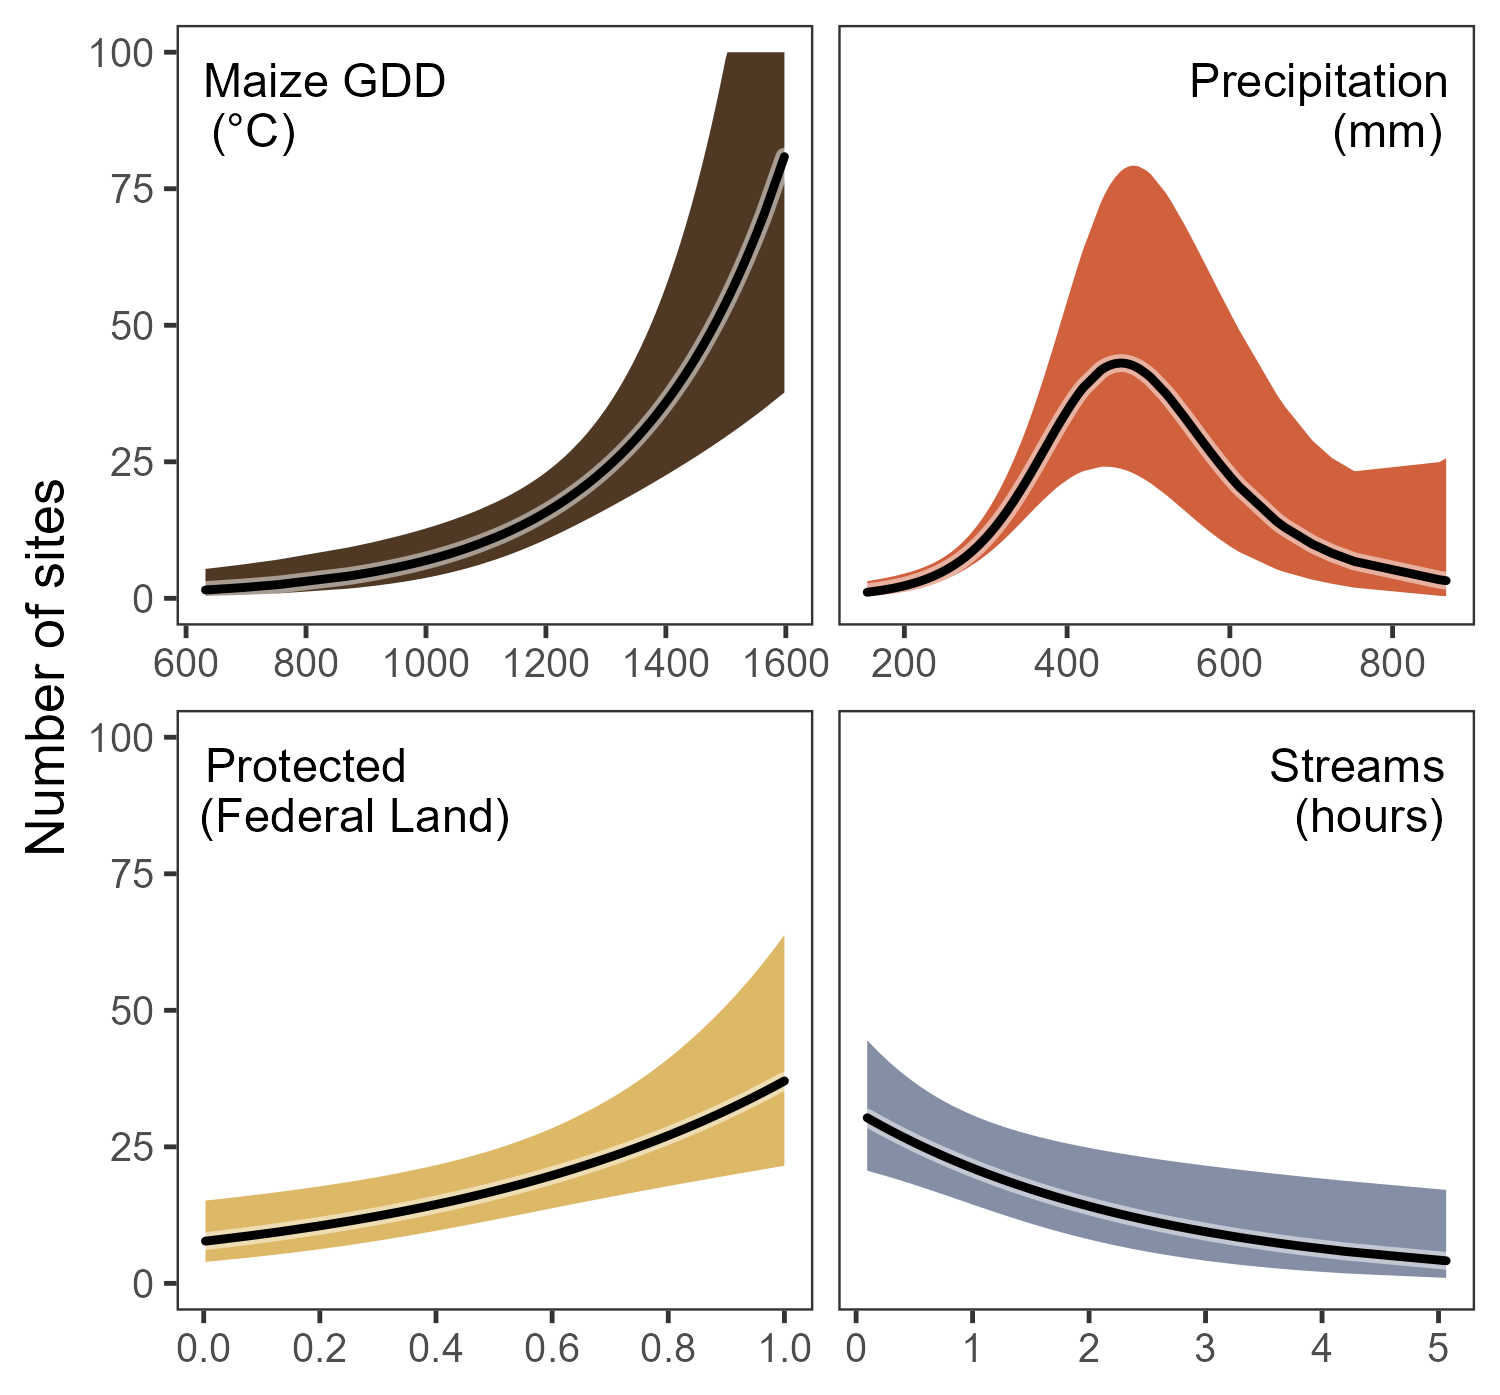
\includegraphics[width=5in,height=\textheight]{../figures/marginal_response.png}

}

\caption{\label{fig-responses}Marginal response plots. Each plot shows
the response of site counts to changes in a target covariate while
holding all other variables at their mean.}

\end{figure}

\hypertarget{discussion}{%
\section{Discussion}\label{discussion}}

Our results indicate that Fremont maize farmers generally preferred
warmer watersheds with longer growing seasons, moderate levels of
precipitation (in the range of 400-600 mm), and greater access to
perennial streams, as shown by the marginal response plots in Fig. 3.
While site counts exhibit a positive linear response to maize GDD, for
maize has an upper threshold temperature at which point it no longer
grows. Plus, increased temperatures trade-off with water availability,
with warmer conditions being better for plant growth but at the same
time increasing water demand on the plant to keep up with growth
\citep{ramankutty2002}. The linear relationship between site counts and
maize GDD is, thus, relative to the observed distribution of that
variable within the study area and should not be used to generalize to a
larger geographic extent.

Another curious result of our analysis is that site counts do not
increase linearly as a function of precipitation, but instead decline
after 500 mm. We believe this is likely an artifact of trade-offs
related to elevation, specifically the trade-off between precipitation
and temperature. We discuss this more below, along with other important
implications our results have for the regional prehistory of the eastern
Great Basin, particularly for the spread and eventual collapse of maize
agriculture.

\hypertarget{a-goldilocks-zone}{%
\subsection{A Goldilocks Zone?}\label{a-goldilocks-zone}}

Provided that the trade-off between precipitation and temperature is
driven largely by elevation in this region, it would seem likely that
the western Fremont chose site locations at elevations that maximized
agricultural suitability, as evidenced by the estimated distribution of
sites across watersheds (see Fig. 4), though we caution that watersheds
are coarse grained units of analysis. Given the topography of the study
area, this trade-off would also suggest that areas suitable for maize
agriculture take the form of a thin band around the lower slopes of
mountain ranges (or lower canyons in the Uintas). Such a band would be
akin to a Goldilocks zone for maize agriculture (Yaworsky et al, this
issue), a place where the optima for GDD and precipitation overlap,
though we should not make too much of this idea, for it is an area of
overlap for continuous ecological gradients, not a region demarcated by
anything like a perfect line. It also must be emphasized that what
matters most for maize agriculture is not necessarily where
precipitation falls, but where it accumulates once it enters the
streamflow network. Of course, that will largely be a function of
elevation in this region, or changes in elevation, so it will still be
in proximity to the Goldilocks zone, though perhaps not perfectly
coincident with it. At any rate, given these considerations, it would
perhaps be more accurate to characterize the trade-off confronting the
Fremont as one between what we might call water availability (including
general precipitation across the streamflow network, water runoff,
proximity to perennial surficial sources, and irrigation potential,
among other things) and temperature (including, but not limited to, the
length of the growing season and the number of frost-free days).

\hypertarget{irrigation-and-the-maize-farming-niche}{%
\subsection{Irrigation and the Maize Farming
Niche}\label{irrigation-and-the-maize-farming-niche}}

Based on previous research \citep{benson2011, adams2006, bellorado2010},
Bocinsky and Kohler \citep{bocinsky2014} place minimum thresholds for
precipitation and maize GDD at 300 mm and 1000°C GDD, respectively.
Importantly, these are thresholds for dry-farming, which is typically
defined as farming free of irrigation
\citep{benson2011, cordell2012, varien1999}, so they can be loosely
interpreted as minimum temperature and precipitation levels required to
grow maize through nothing more than planting and harvesting. The right
panel in Figure~\ref{fig-thresholds} shows the watersheds whose median
values for maize GDD and precipitation over the Fremont sequence are
above those values. This is similar to Bocinsky's concept of
``refugia,'' but rather than calculate the proportion of years in niche,
we are using median values, so refugia are defined here as watersheds
that spend at least half the Fremont sequence in the rain-fed maize
farming niche (\(\geq\) 500 years, in this case).

\begin{figure}

{\centering 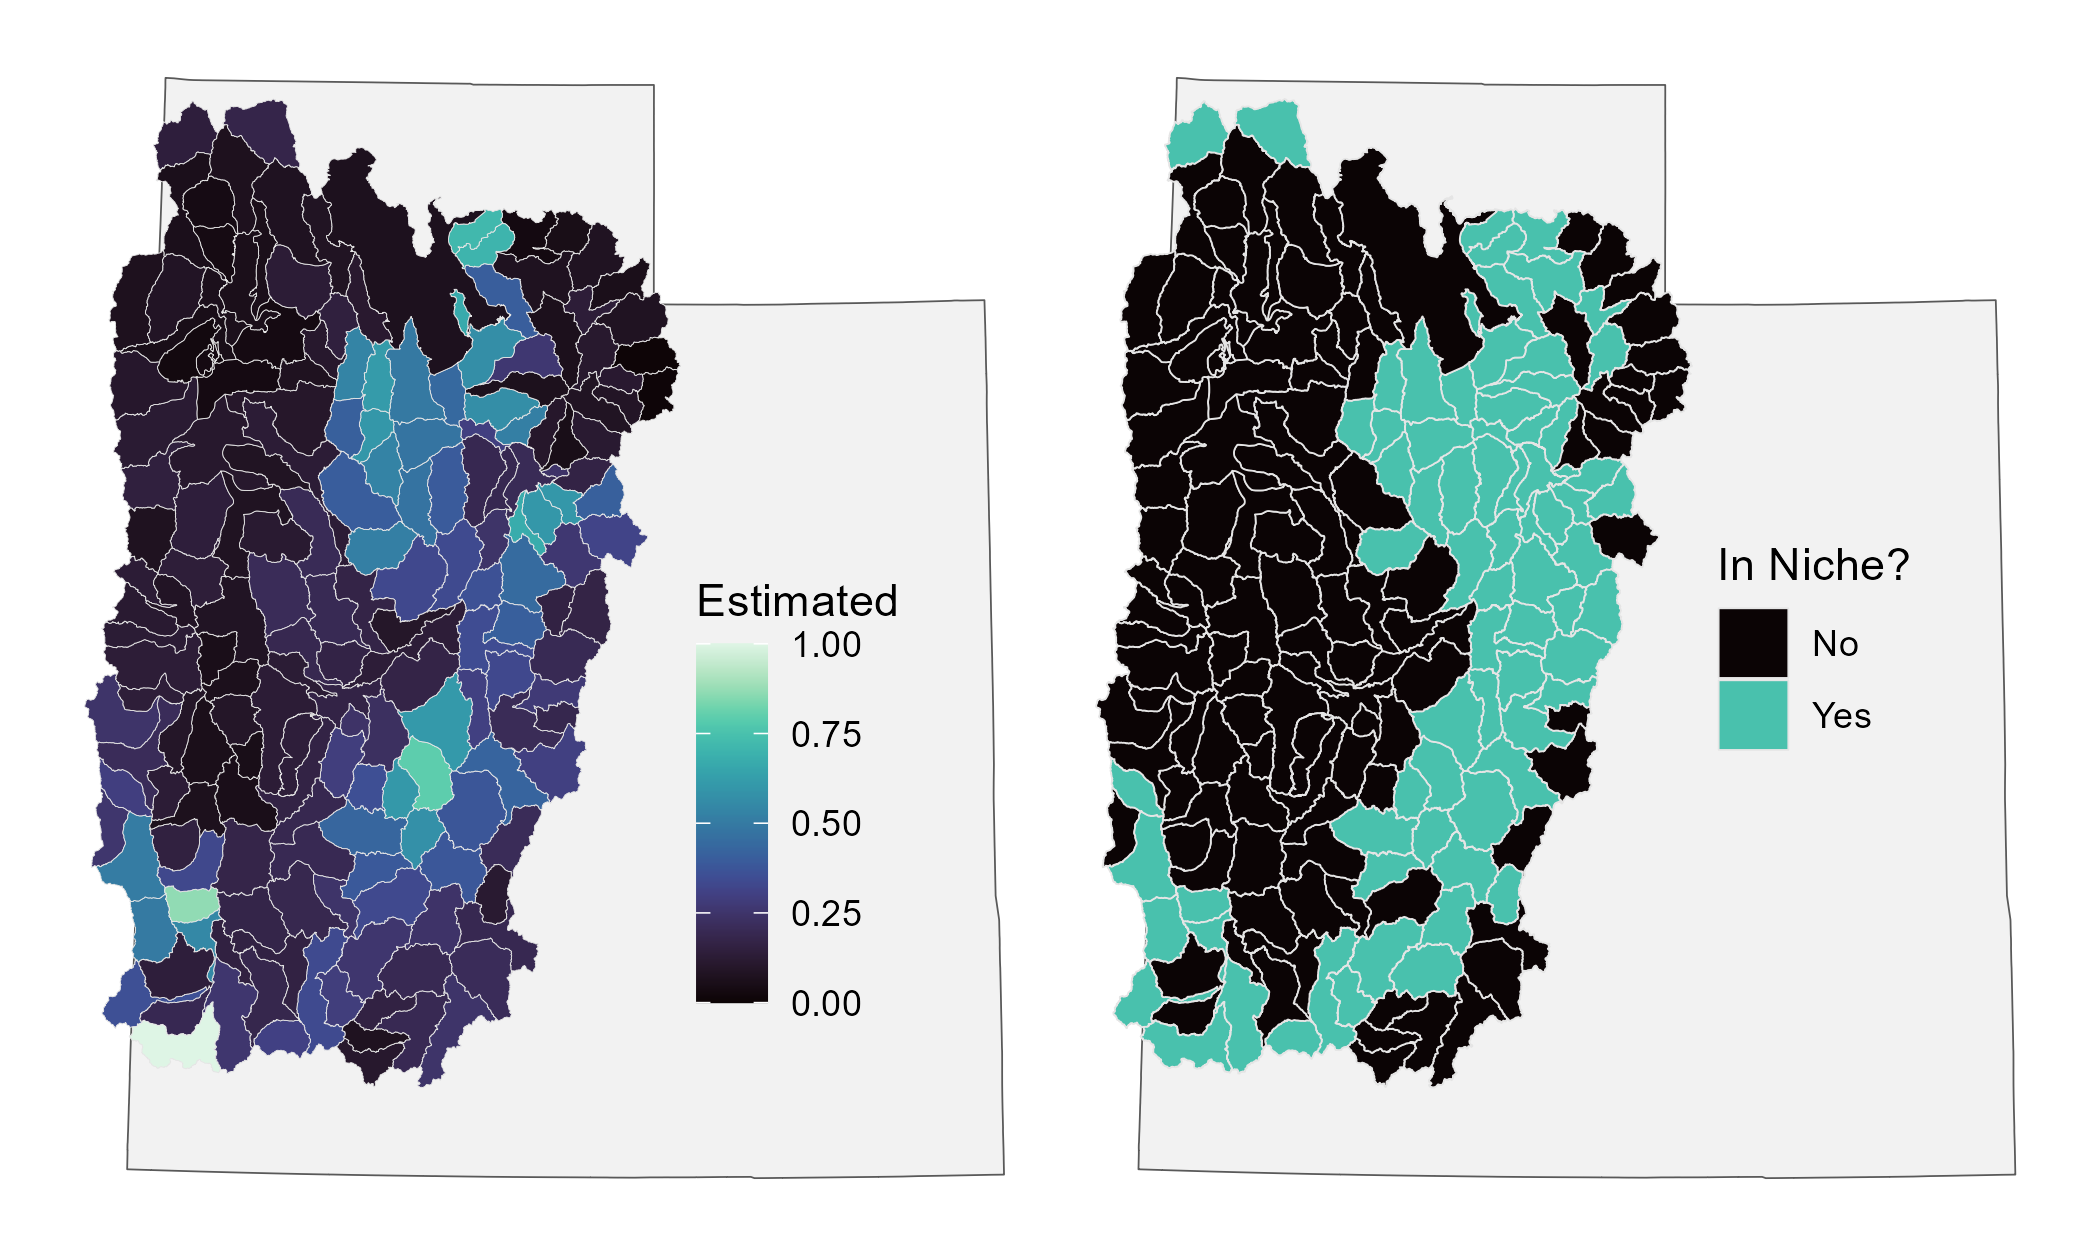
\includegraphics[width=6in,height=\textheight]{../figures/threshold_map.png}

}

\caption{\label{fig-thresholds}The map on the left shows the relative
density of feature-weighted site counts as estimated by the model, with
lighter colors representing larger relative densities, darker colors
representing smaller relative densities. The map on the right shows
which watersheds are in the rain-fed maize farming niche for at least
half of the Fremont sequence. The light green color indicates those that
are in the niche.}

\end{figure}

It appears that these models tend to agree on the best watersheds for
maize farming, though there are some notable exceptions. The western
slopes of the Stansbury Range in the north central part of the study
area and parts of the Parowan Valley and surrounding areas in the
southeast part of the study area are estimated by our model to have
non-negligible relative densities, but they fall outside of the niche.
Other areas, like much of the Salt Lake valley appear to be in the
niche, but are estimated by our model to have relatively low densities.
These discrepancies are at least partially explained by limitations of
our methodology. For one thing, including the proportion of federal land
as a covariate is a very crude way of accounting for sampling bias, so
our model might not be picking up on the fact that the Salt Lake valley
was actually a highly suitable area for maize agriculture, as evidence
to that effect has largely been destroyed. The discrepancy may also be
explained by the fact that we have aggregated to the watershed level,
thus obscuring important environmental variation across both the
landscape in general and site locations in particular. Were we to build
a model of the disaggregated data, we would likely find that many
agricultural sites do, in fact, fall in the rain-fed maize agricultural
niche, even if the watersheds that contain them do not.

But setting aside those methodological issues, some much more
interesting explanations may be offered, at least from the perspective
of theory. In particular, the spatial covariance structure in our model
may be picking up on the structure of the streamflow network,
specifically the accumulation of water run-off as a function of slope.
This would suggest that if there are more people in one watershed, there
should be more more people in the downstream watershed, too, at least
relative to other watersheds with similar precipitation and GDD values.
In the language of the IFD model, the suitability of the watershed
habitat should propagate through the streamflow network. Exploring that
intuition in a more systematic way, however, would require much more
careful consideration of streamflow. Unfortunately, that is well beyond
the scope of the current paper.

Still, the distribution of the rain-fed niche may offer additional
insights. Consider the fact that of the 183 watersheds in the study
area, 87\% (n=159) have median GDD values greater than 1000°C, but only
54\% (n=98) have median precipitation values above 300 mm, and a scant
40\% (n=74) meet both requirements. This would suggest that
precipitation is the primary limiting factor when it comes to the choice
of watersheds in which to dry farm, for there are many more watersheds
that meet the minimum GDD requirements than meet the minimum
precipitation requirements. One important implication of this is that
dry farming would have been very nearly impossible across most of the
study area over the Fremont sequence and irrigation more or less
necessary. We note that even within the niche, which we have defined
somewhat liberally as those watersheds that are included for at least
half the Fremont sequence, irrigation would almost certainly have been a
necessity \citep{boomgarden2019, matson1990, spangler2010}. Of course,
the type and intensity of irrigation would probably differ between
sites, with more intensive irrigation occurring where there is less
precipitation and less intensive irrigation where there is more
precipitation, whether that precipitation falls in the watersheds
themselves or in the upstream watersheds that feed into them.

\hypertarget{the-spread-of-maize-agriculture}{%
\subsection{The Spread of Maize
Agriculture}\label{the-spread-of-maize-agriculture}}

Our results comport with previous work suggesting that maize farmers in
the eastern Great Basin preferentially targeted a certain elevation band
that coincides with alluvial fans, forming a rim around the lower slopes
of mountains and ridges on or near important drainages and floodplains.
The ruggedness and aridity of this region led to extreme
circumscription, with the costs of intensive farming outside these areas
being so severe as to render that alternative virtually unsustainable.
For maize farmers, the Great Basin should, thus, have the look and feel
of an island biogeography, with mountains rising up like islands out of
an ocean of desert sand and sagebrush.

To account for the timing and tempo of island colonization among food
producers in Oceania, \citep{kennett2006} offer an extension of the IFD
framework that might actually apply to the Great Basin. Their model
depends crucially on the potential for farming populations to introduce
economies of scale or Allee effects, with suitability increasing with
increasing population at low densities. They also assume that
individuals will prefer nearer habitats to those that are farther away,
under the assumption that greater distances impose greater settlement
costs, all else being equal. Together, these assumptions suggest a
pulsating pattern of maize spread into the North American Southwest,
with maize agriculture growing, then spreading, growing, then spreading,
as appears to have happened in Oceania.

This need not be a wholesale movement or adoption of agricultural
practices, either. \citep{madsen1998} argue that Fremont subsistence
largely varies along two dimensions: levels of residential mobility and
levels of cultigen adoption. While some were more mobile, moving from
isolated patch to isolated patch, others were more sedentary, typically
tethered to a productive wetland or riparian area. As local populations
increase, the benefits of increased sedentism and cultigen adoption
would slowly begin to outweigh the benefits of a more mobile and
foraging-centered diet. According to our model, individuals moving in
this direction would tend to concentrate more of their time and energy
in the maize farming niche. This would then have the effect of
increasing population size within a smaller area, possibly leading to
Allee effects, which would invite further sedentism from those in the
surrounding area. Following this logic, the patchy adoption of
agriculture makes more sense. The degree and speed with which it occurs
is simply a function of how fast habitat quality declines and how
quickly populations grow.

\begin{figure}

{\centering 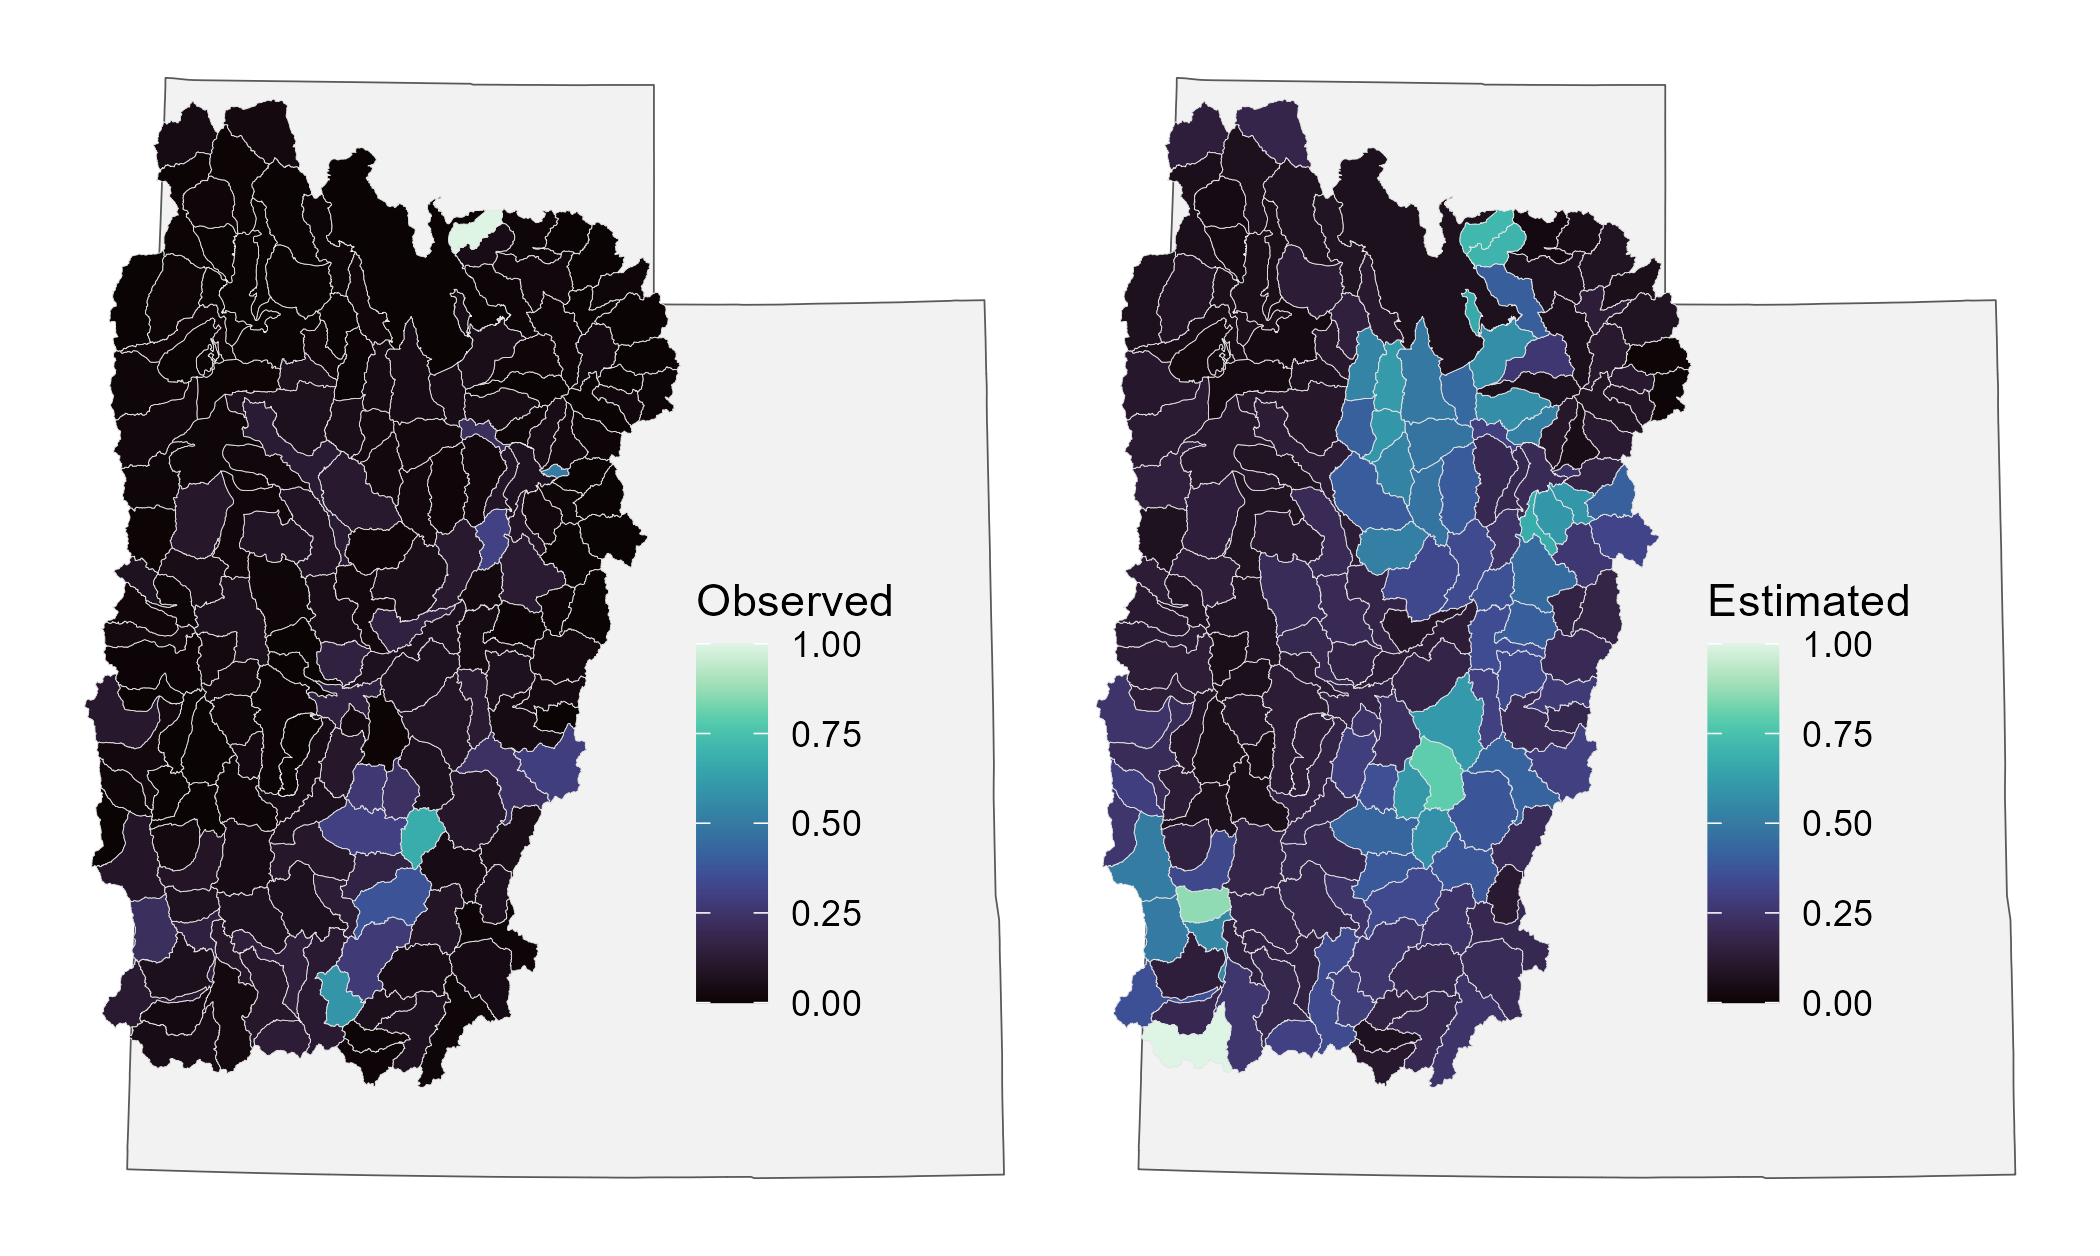
\includegraphics[width=6in,height=\textheight]{../figures/model-map.png}

}

\caption{\label{fig-model-map}Geographic distribution of Fremont sites
across watersheds. The left panel shows the relative density derived
from observed site counts, and the right panel shows the relative
density from the estimated site counts.}

\end{figure}

\hypertarget{the-collapse-of-maize-agriculture}{%
\subsection{The Collapse of Maize
Agriculture}\label{the-collapse-of-maize-agriculture}}

After farming these regions successfully for over a thousand years, the
Fremont began an abrupt process of abandonment starting around 700 years
BP. The cause of this event is still a matter of some dispute, though a
growing consensus appears to be coalescing around climatic changes
driving severe reductions in agricultural productivity
\citep{benson2007, spangler2019, thomson2019, thomson2020, finley2020}.
We follow \citep{lindsay1986} in thinking this was likely owing to
climatic events that, in effect, tore the Goldilocks zone apart, pulling
higher temperatures further down in elevation and pushing higher
precipitation levels further up.

Lindsay suggests that the end of the Medieval Warm Period may have been
responsible for this decoupling, as it involved higher temperatures and
more growing-season precipitation owing to the northward intrusion of
summer monsoons. This period lasted from roughly 1,000 to 600 years BP
\citep{grayson2011, graumlich1993}, so it does coincide with the height
of the Fremont complex. Given the logic of IFD, this likely led to
population spillovers into less suitable habitats \citep{codding2021}.
However, given the extreme circumscription we have highlighted in the
Great Basin, the available alternatives would have been limited,
potentially leading to increasing population packing across all habitats
during this time, thus making the Fremont especially sensitive to
climatic downturns.

The well-documented megadrought at the end of the thirteenth century
\citep{cook2004} would have been catastrophic in this context, reducing
precipitation levels across the region \citep{benson2007}, but also
leading to reductions in water accumulation within the streamflow
network. So, just as temperatures are beginning to cool, precipitation
levels collapse. By extension, this would have decreased overall water
availability and, thus, the potential for irrigation. Opportunities for
the Fremont to recover from such a drought would have been limited, too,
as the end of the Medieval Warm Period was also the beginning of the
Little Ice Age, a time during which conditions were generally colder and
wetter \citep{mann2009}, further pulling apart the Goldilocks zone upon
which the Fremont so long depended.


  \bibliography{bibliography.bib}


\end{document}
